\subsection{Memory and Execution-Time Profiling}
\label{subsec:pmc-results-memory-and-execution-time-profiling}

This section examines raw memory and execution-time measurements.
The goal is to understand how input shape influences resource demand before applying predictive modeling.
While full feature selection results are discussed later (Section~\ref{subsec:pmc-results-feature-selection-experiments}), the clear dominance of the \emph{volume} feature\textemdash defined as $\text{inlines} \times \text{xlines} \times \text{samples}$\textemdash motivates its early focus in the analysis.

\subsubsection{Linear Trends and Variability}
\label{subsec:linear-trends-and-variability}

Figure~\ref{fig:peak_memory_facet} illustrates that peak memory usage scales approximately linearly with volume.
The Envelope, \ac{GST3D}, and Gaussian Filter operators exhibit similar growth patterns, albeit with different slopes and variabilities.
Larger volumes lead to more consistent memory consumption, whereas smaller volumes show higher \ac{CV} due to overhead fluctuations such as interpreter startup or I/O buffering.

\begin{figure*}[htbp]
    \centering
    \begin{subfigure}[t]{0.32\textwidth}
        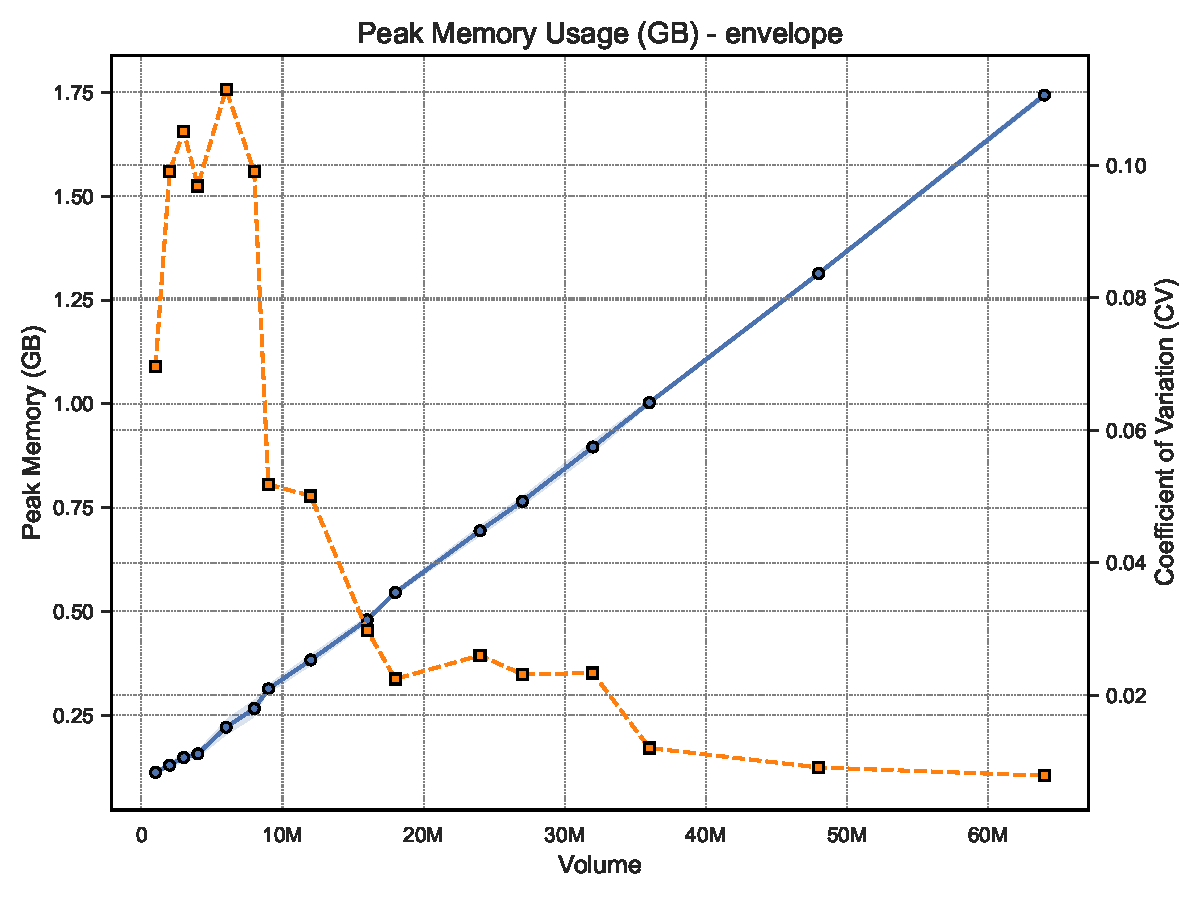
\includegraphics[width=\textwidth]{assets/images/05/peak_memory_by_volume_envelope}
        \caption{Envelope}
    \end{subfigure}
    \hfill
    \begin{subfigure}[t]{0.32\textwidth}
        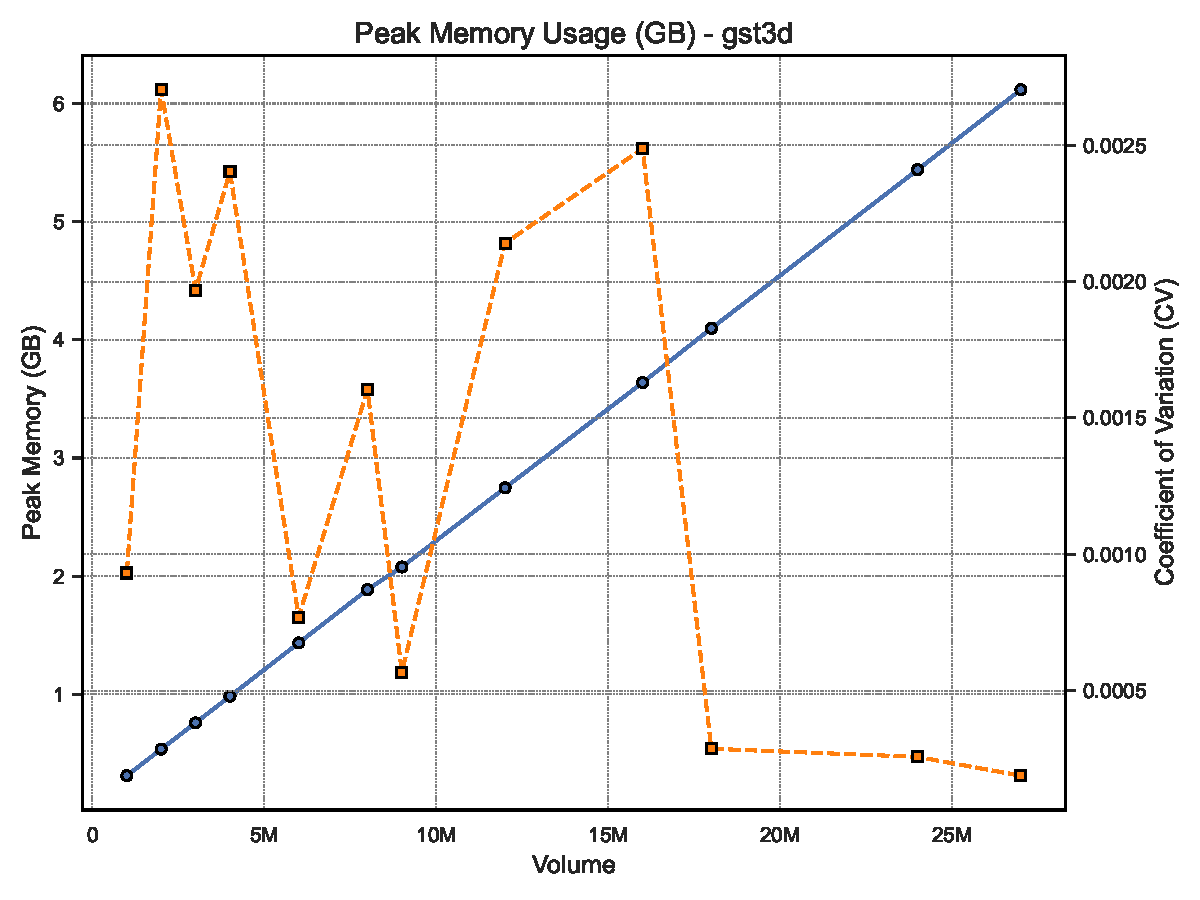
\includegraphics[width=\textwidth]{assets/images/05/peak_memory_by_volume_gst3d}
        \caption{\ac{GST3D}}
    \end{subfigure}
    \hfill
    \begin{subfigure}[t]{0.32\textwidth}
        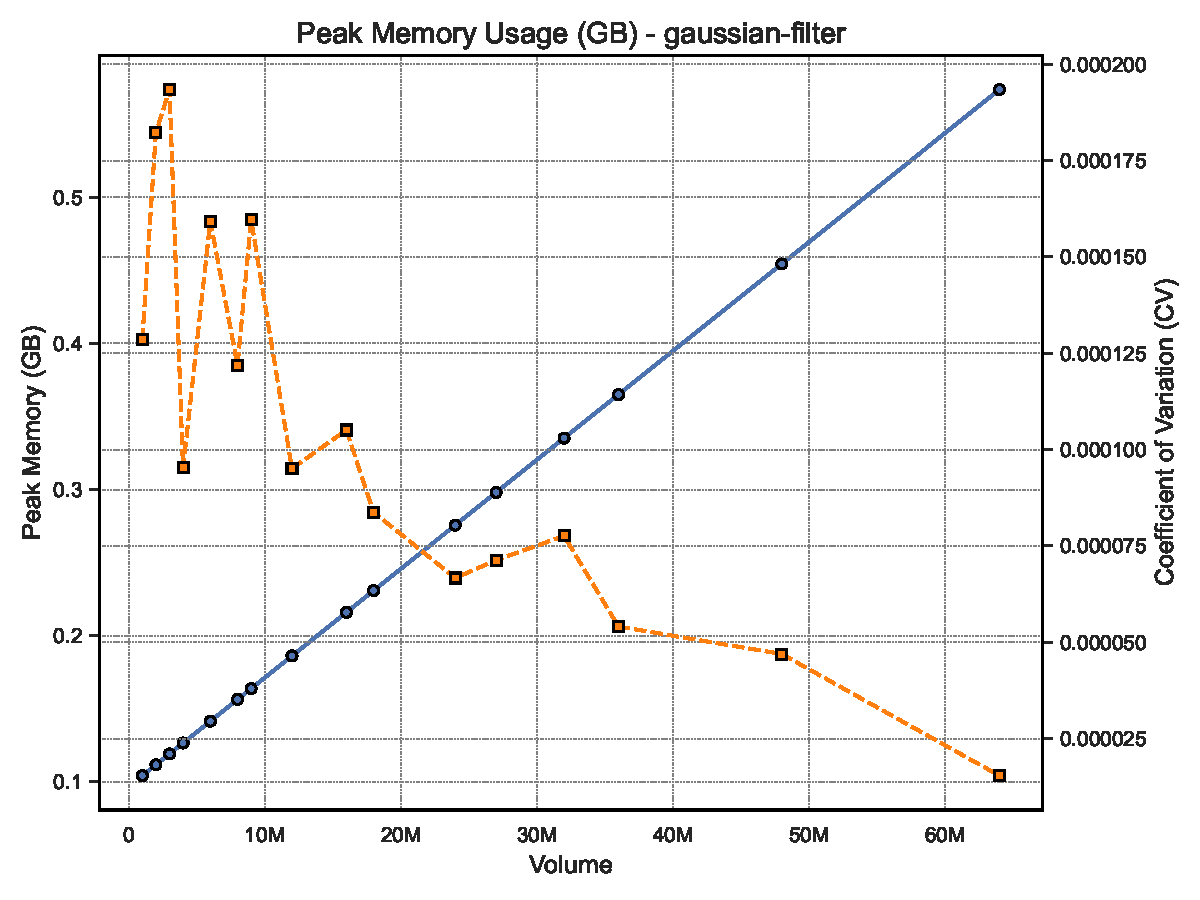
\includegraphics[width=\textwidth]{assets/images/05/peak_memory_by_volume_gaussian-filter}
        \caption{Gaussian Filter}
    \end{subfigure}
    \caption{Peak memory usage vs. $Volume~(\text{inlines} \times \text{xlines} \times \text{samples})$ for Envelope, \ac{GST3D}, and Gaussian Filter. Each operator displays approximate linear scaling. Variability is higher in smaller volumes.}
    \label{fig:peak_memory_facet}
\end{figure*}

Execution times follow a similar trend.
Figure~\ref{fig:execution_time_by_volume_facet} confirms a near-linear increase with volume for all three operators.
This reinforces that input shape, especially total volume, is the dominant factor influencing resource usage in these seismic kernels.

\begin{figure*}[htbp]
    \centering
    \begin{subfigure}[t]{0.32\textwidth}
        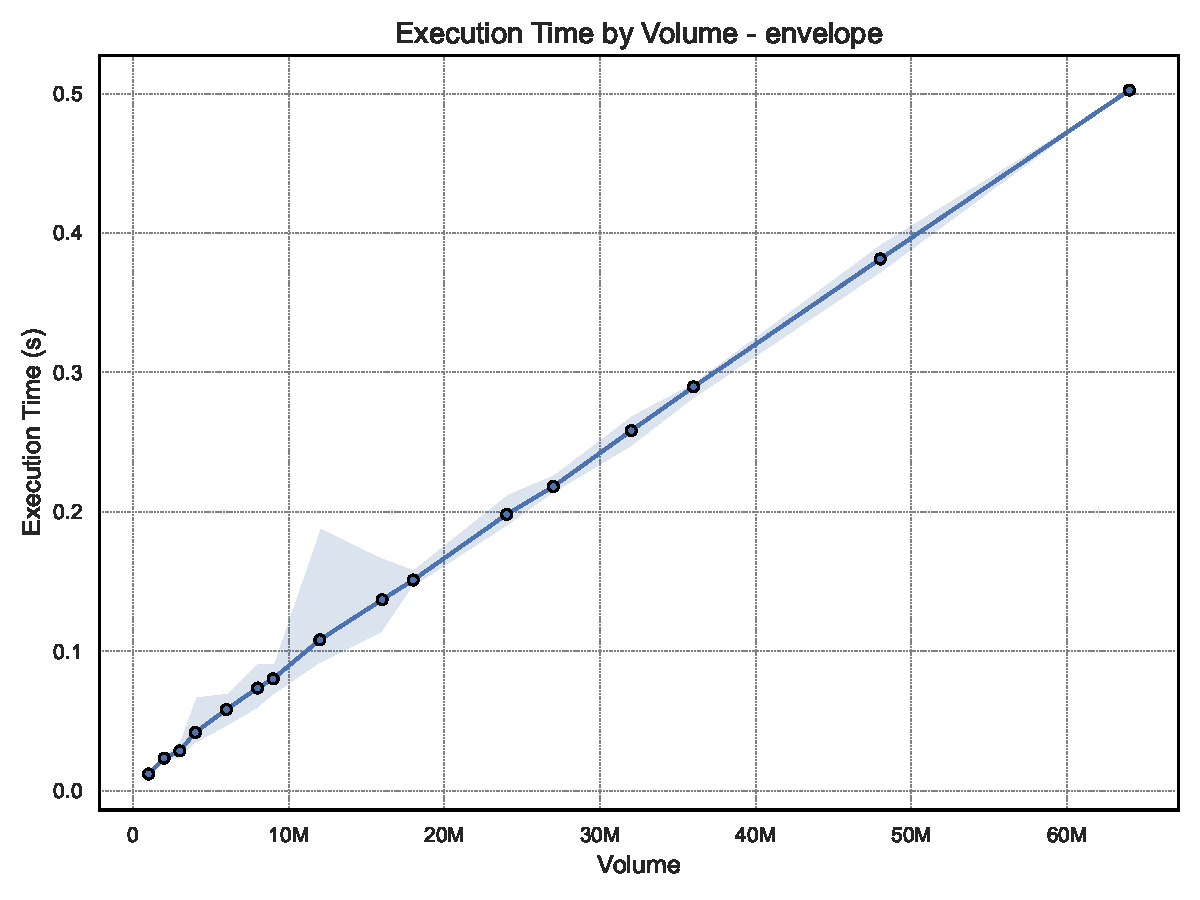
\includegraphics[width=\textwidth]{assets/images/05/execution_time_by_volume_envelope}
        \caption{Envelope}
    \end{subfigure}
    \hfill
    \begin{subfigure}[t]{0.32\textwidth}
        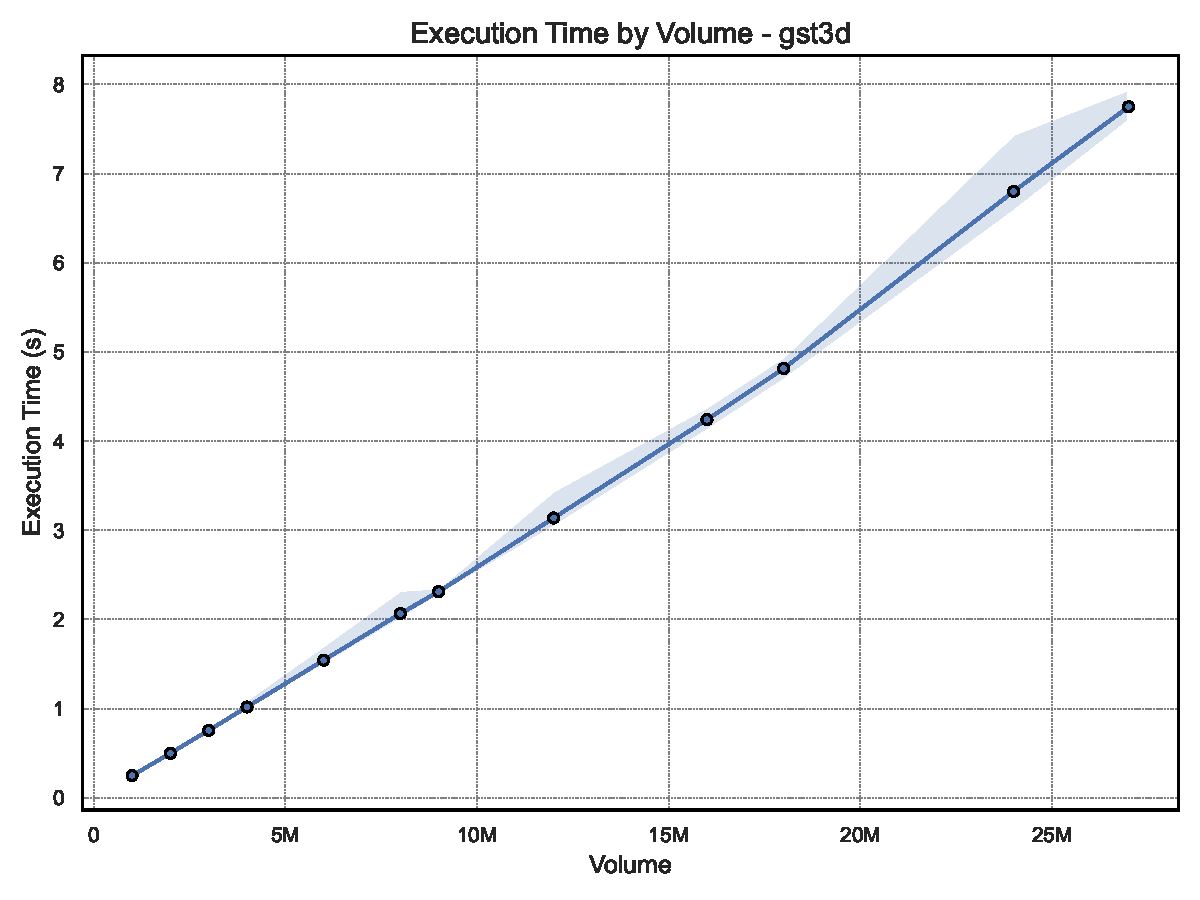
\includegraphics[width=\textwidth]{assets/images/05/execution_time_by_volume_gst3d}
        \caption{\ac{GST3D}}
    \end{subfigure}
    \hfill
    \begin{subfigure}[t]{0.32\textwidth}
        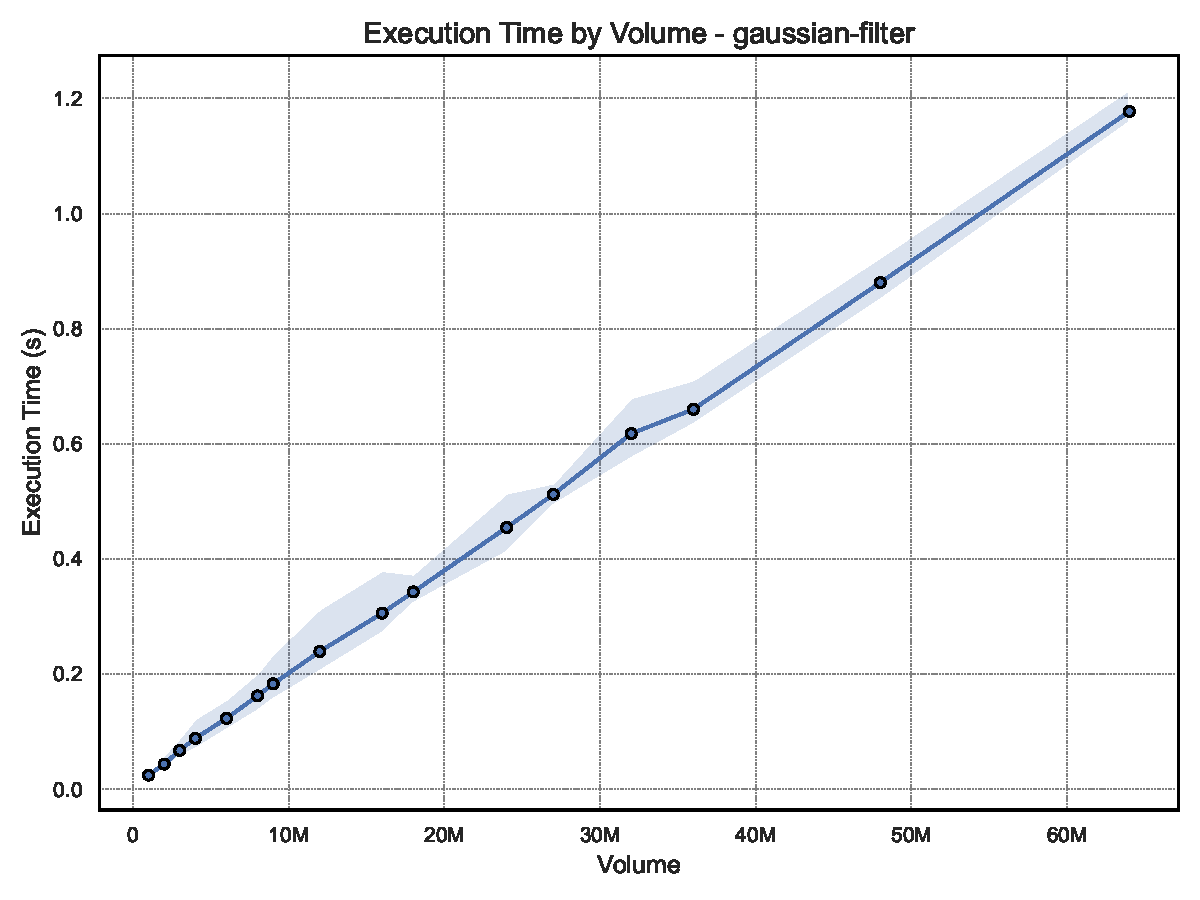
\includegraphics[width=\textwidth]{assets/images/05/execution_time_by_volume_gaussian-filter}
        \caption{Gaussian Filter}
    \end{subfigure}
    \caption{Execution time by volume. Each operator demonstrates a growth trend, suggesting that volume captures most of the computational effort.}
    \label{fig:execution_time_by_volume_facet}
\end{figure*}

\subsubsection{Execution Time Distributions and Scaling Factor}
\label{subsec:execution-time-distributions-and-scaling}

Figure~\ref{fig:ex_peak_mu_facet}(a)--(c) aggregate execution time and peak memory usage for all operators.
Since we can see a cler linear pattern, table~\ref{tab:scaling_slopes_summary} lists the slope and $R^2$ values considering a linear regression fit.
\ac{GST3D} exhibits the steepest slope, followed by Envelope and then Gaussian Filter, indicating increasingly efficient memory usage.

\begin{figure*}[htbp]
    \centering
    \begin{subfigure}[t]{0.49\textwidth}
        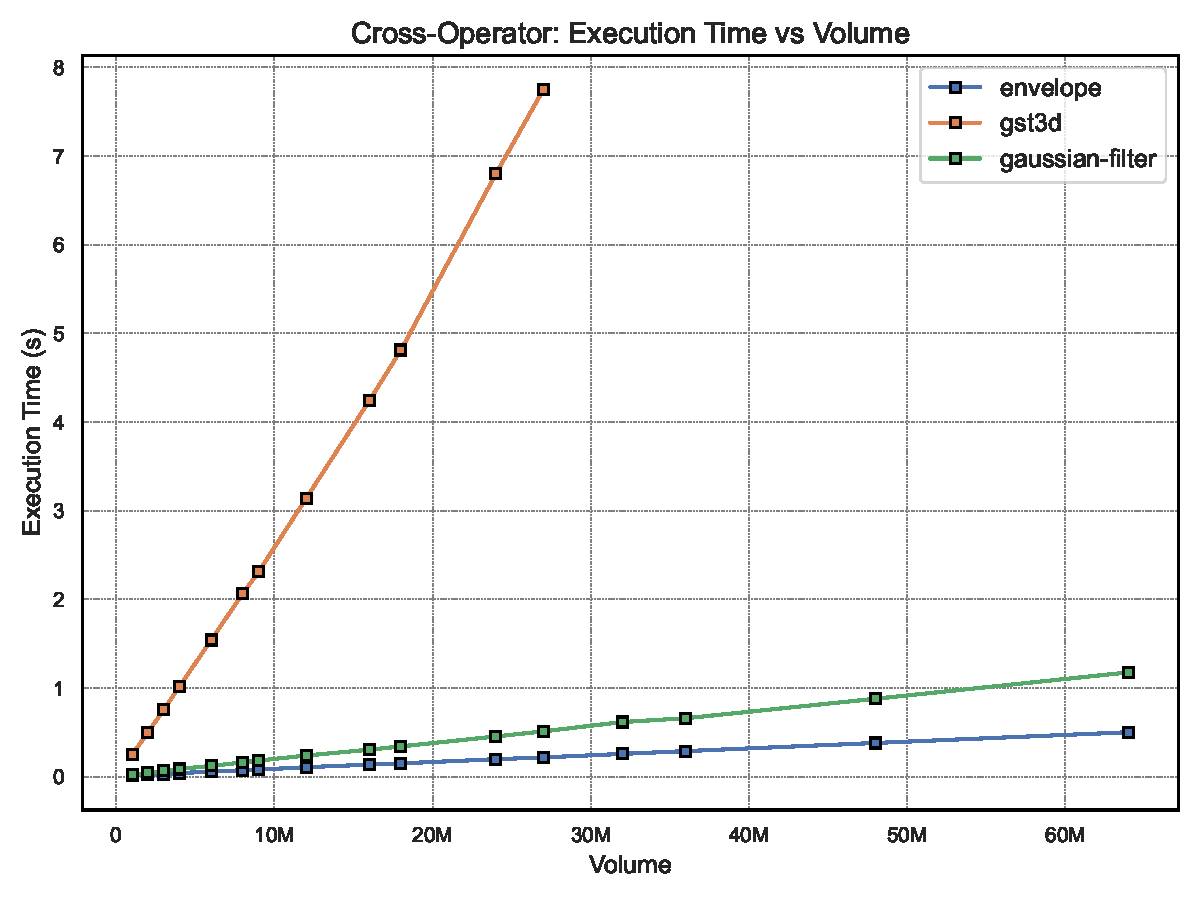
\includegraphics[width=\textwidth]{assets/images/05/cross_execution_time_by_volume}
        \caption{Execution time vs. volume}
    \end{subfigure}
    \hfill
    \begin{subfigure}[t]{0.49\textwidth}
        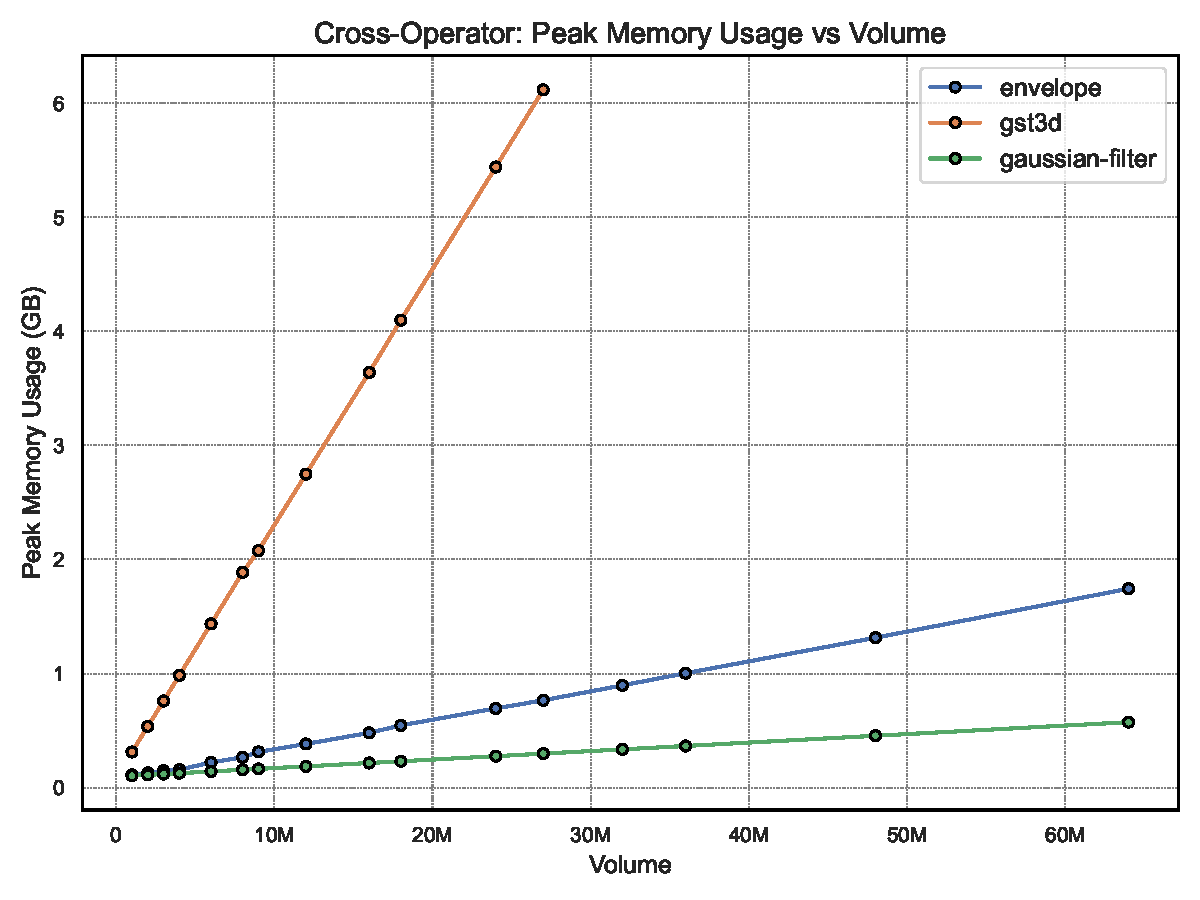
\includegraphics[width=\textwidth]{assets/images/05/cross_peak_memory_by_volume}
        \caption{Peak memory vs. volume}
    \end{subfigure}
    \caption{Combined memory and execution time vs. volume for all operators. All metrics scale nearly linearly.}
    \label{fig:ex_peak_mu_facet}
\end{figure*}

\begin{table}[htbp]
    \centering
    \begin{tabular}{lcc}
        \hline
        \textbf{Operator} & \textbf{Memory Slope (GB/volume)} & \textbf{$R^2$} \\
        \hline
        Envelope          & 0.000027                          & 0.996          \\
        \ac{GST3D}        & 0.000128                          & 0.998          \\
        Gaussian Filter   & 0.000011                          & 0.994          \\
        \hline
    \end{tabular}
    \caption{Linear regression slope and $R^2$ for peak memory vs. volume.}
    \label{tab:scaling_slopes_summary}
\end{table}

\subsubsection{Dimension-Specific and Time-Progression Analysis}
\label{subsec:dimension-specific-and-time-progression-analysis}

To isolate the effect of individual dimensions, Figure~\ref{fig:memory_usage_by_configuration_envelope}(a) bins memory usage by each shape parameter.
No dimension dominates, suggesting Envelope memory grows uniformly with input size.

The accompanying heatmap (part~(b)) visually confirms this uniformity: increasing any dimension raises memory similarly.

\begin{figure*}[htbp]
    \centering
    \begin{subfigure}[t]{0.49\textwidth}
        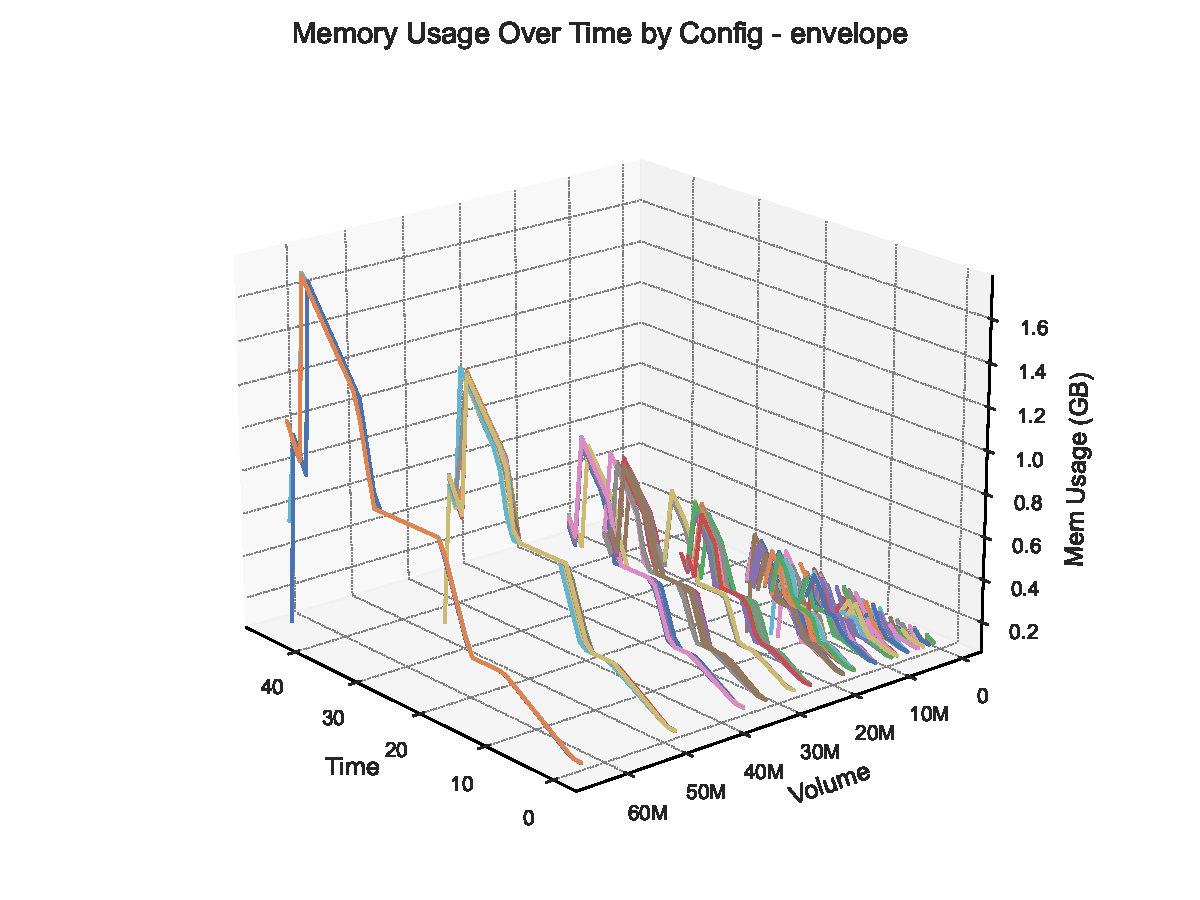
\includegraphics[width=\textwidth]{assets/images/05/memory_usage_by_configuration_envelope}
        \caption{Memory usage by individual dimensions}
    \end{subfigure}
    \hfill
    \begin{subfigure}[t]{0.49\textwidth}
        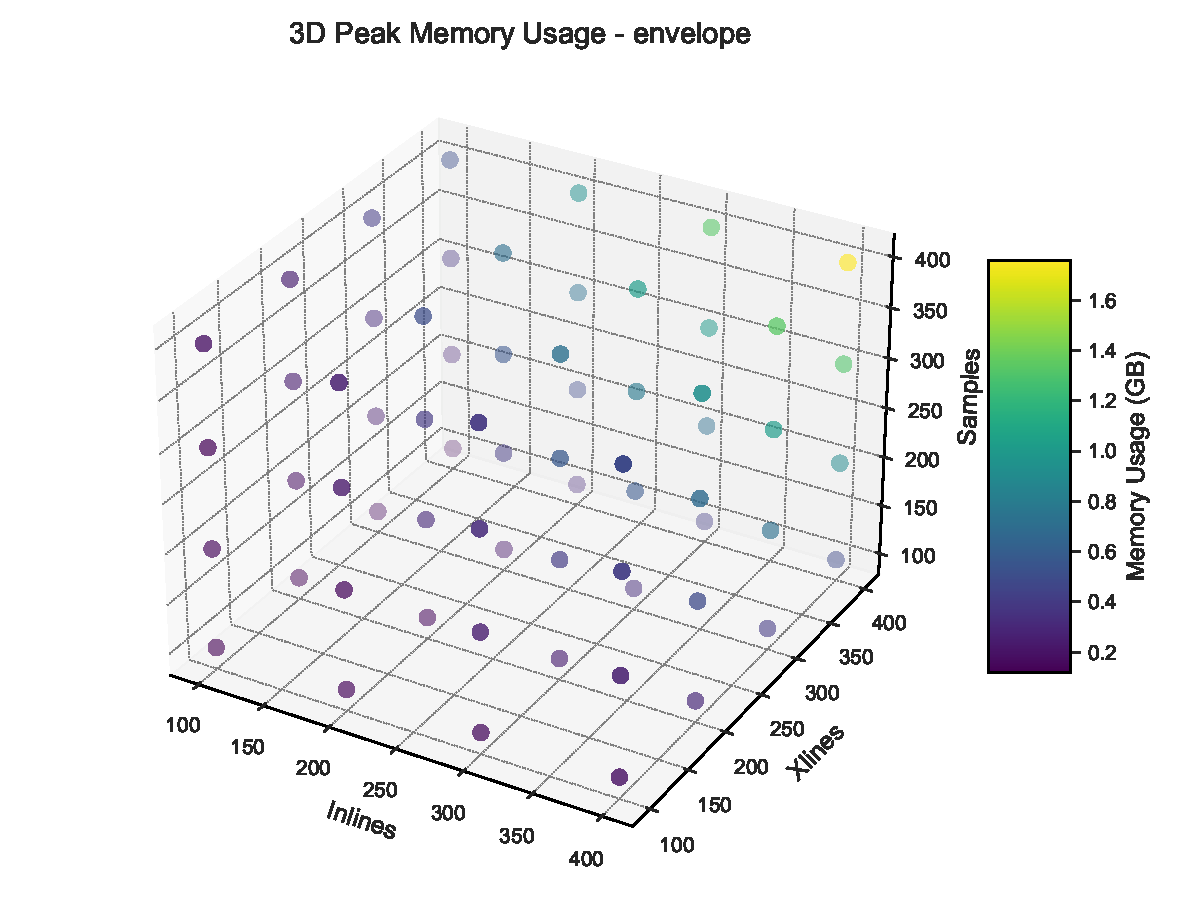
\includegraphics[width=\textwidth]{assets/images/05/memory_usage_inlines_xlines_samples_heatmap_envelope}
        \caption{2D heatmap of shape dimension combinations}
    \end{subfigure}
    \caption{Envelope memory usage decomposed by dimensions. Each axis contributes similarly.}
    \label{fig:memory_usage_by_configuration_envelope}
\end{figure*}

\subsubsection{Memory Safety Margins}
\label{subsec:memory-safety-margins}

Figure~\ref{fig:memory_safety_margin} compares mean and 95th-percentile memory usage.
Significant deviations occur even at fixed volumes, indicating high intra-volume variability likely caused by shape permutations (e.g., $(20,10,10)$ vs. $(10,20,10)$).

This reinforces the need to treat the full shape tuple, not just volume, when assessing outlier behavior.
Nonetheless, models trained on volume alone perform well (Section~\ref{subsec:pmc-results-model-performance-overview}), indicating that these spikes are rare enough to have limited impact on global fit.

\begin{figure*}[htbp]
    \centering
    \begin{subfigure}[t]{0.32\textwidth}
        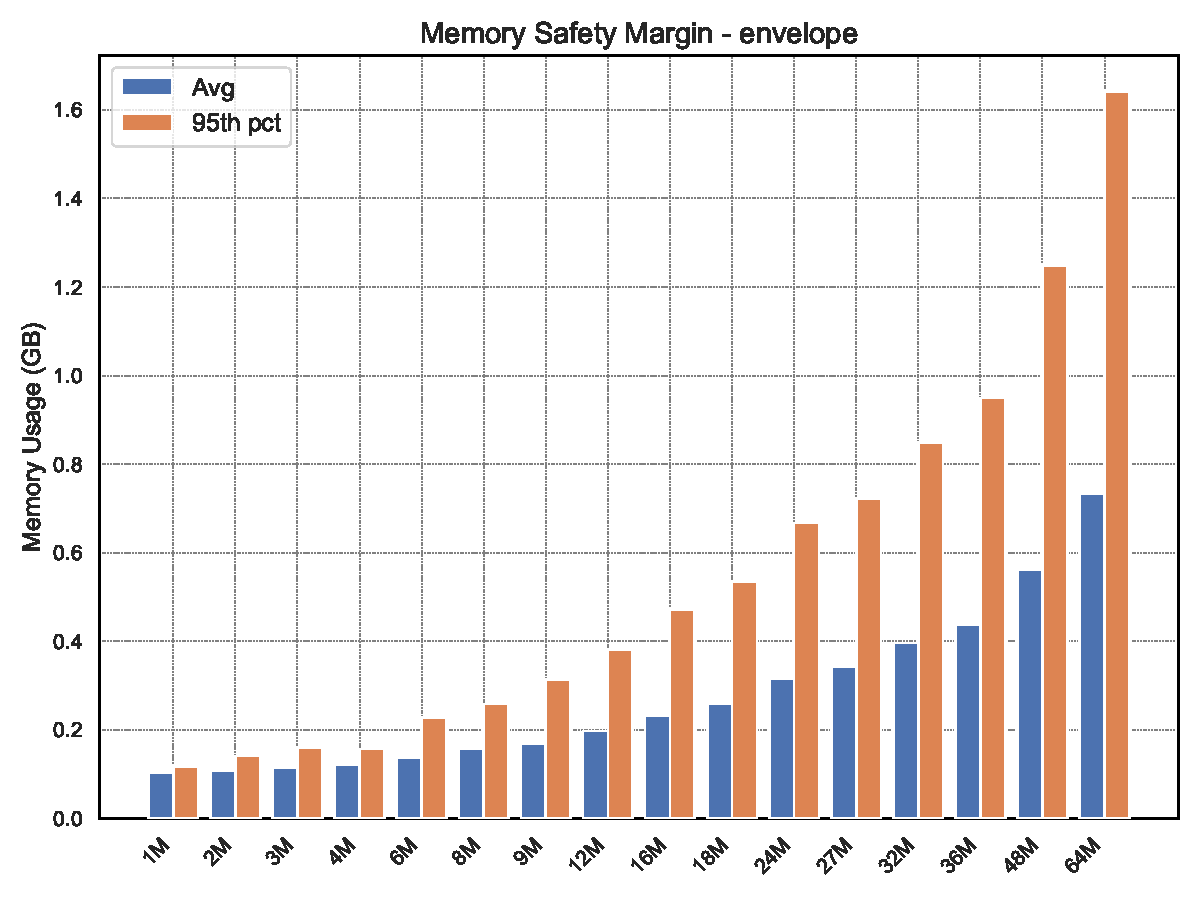
\includegraphics[width=\textwidth]{assets/images/05/memory_safety_margin_envelope}
        \caption{Envelope}
    \end{subfigure}
    \hfill
    \begin{subfigure}[t]{0.32\textwidth}
        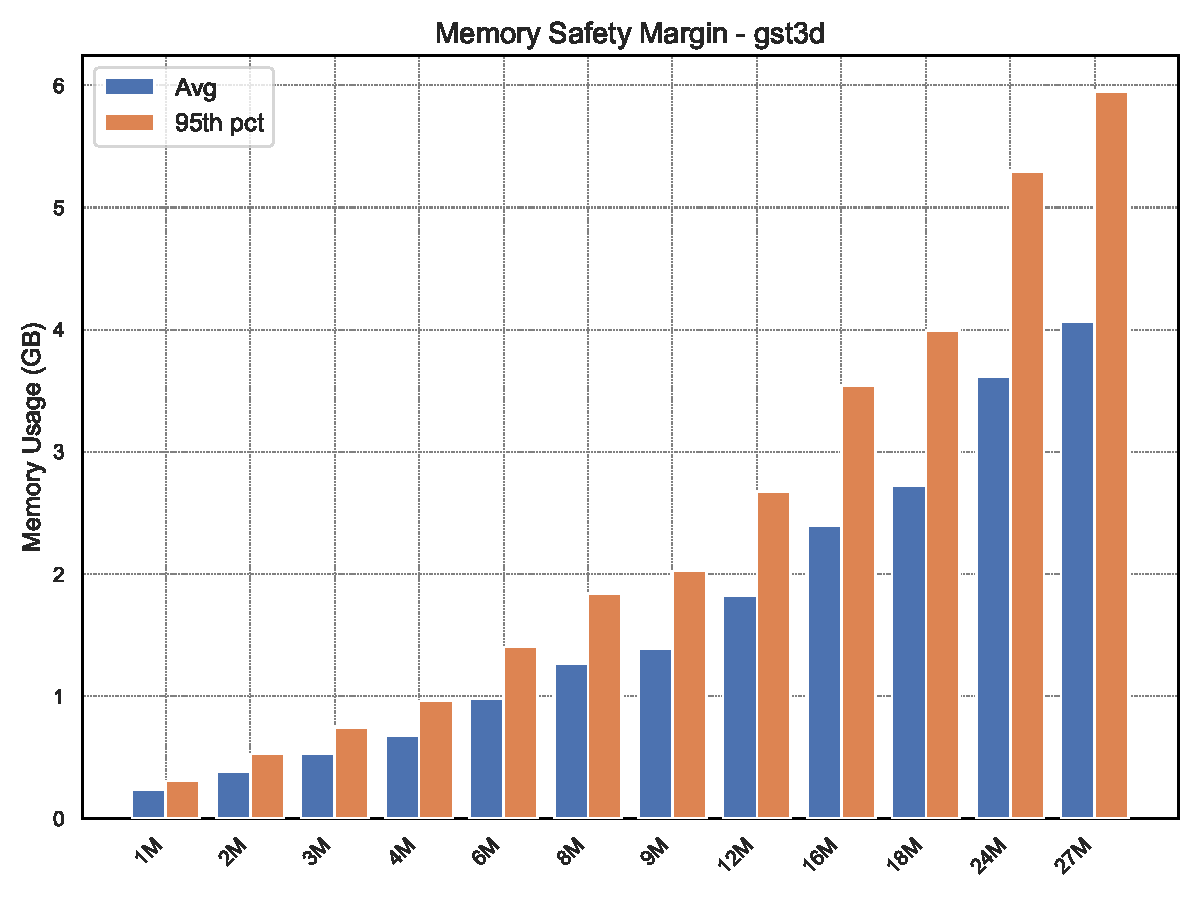
\includegraphics[width=\textwidth]{assets/images/05/memory_safety_margin_gst3d}
        \caption{\ac{GST3D}}
    \end{subfigure}
    \hfill
    \begin{subfigure}[t]{0.32\textwidth}
        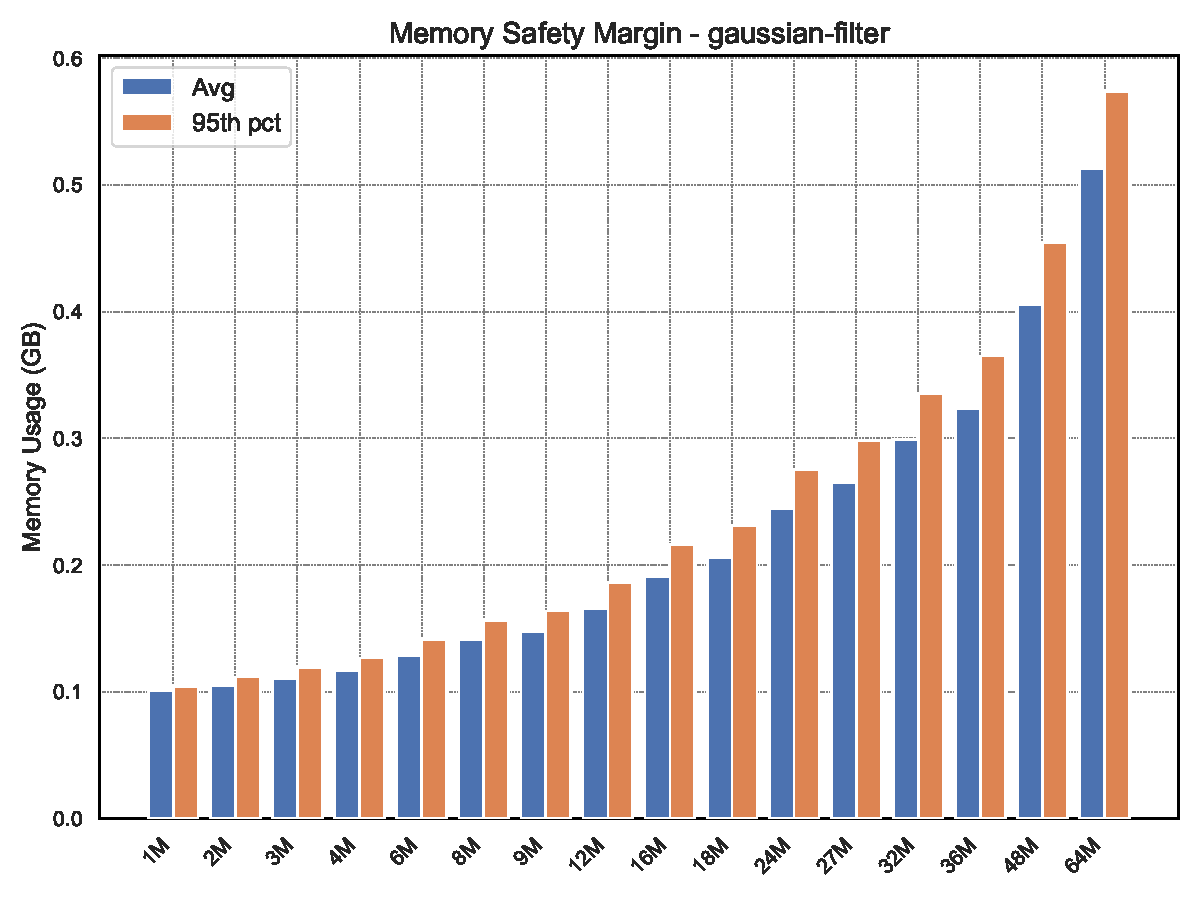
\includegraphics[width=\textwidth]{assets/images/05/memory_safety_margin_gaussian-filter}
        \caption{Gaussian Filter}
    \end{subfigure}
    \caption{Memory safety margins. The 95th-percentile values often exceed the mean, emphasizing the importance of accounting for peak variability.}
    \label{fig:memory_safety_margin}
\end{figure*}

\subsubsection{Dimension Correlations}
\label{subsec:dimension-correlations}

Figure~\ref{fig:memory_vs_dimensions_pairplot_gst3d} presents pairwise plots between \ac{GST3D} memory and each shape parameter.
Memory exhibits strong positive correlation with all three dimensions.

Blue points represent sample values, and red lines are linear regression fits.
Dimension--dimension scatterplots show inverse correlation in some cases, due to how the dataset was constructed.
Nonetheless, when all dimensions increase, memory grows accordingly.

\begin{figure}[htbp]
    \centering
    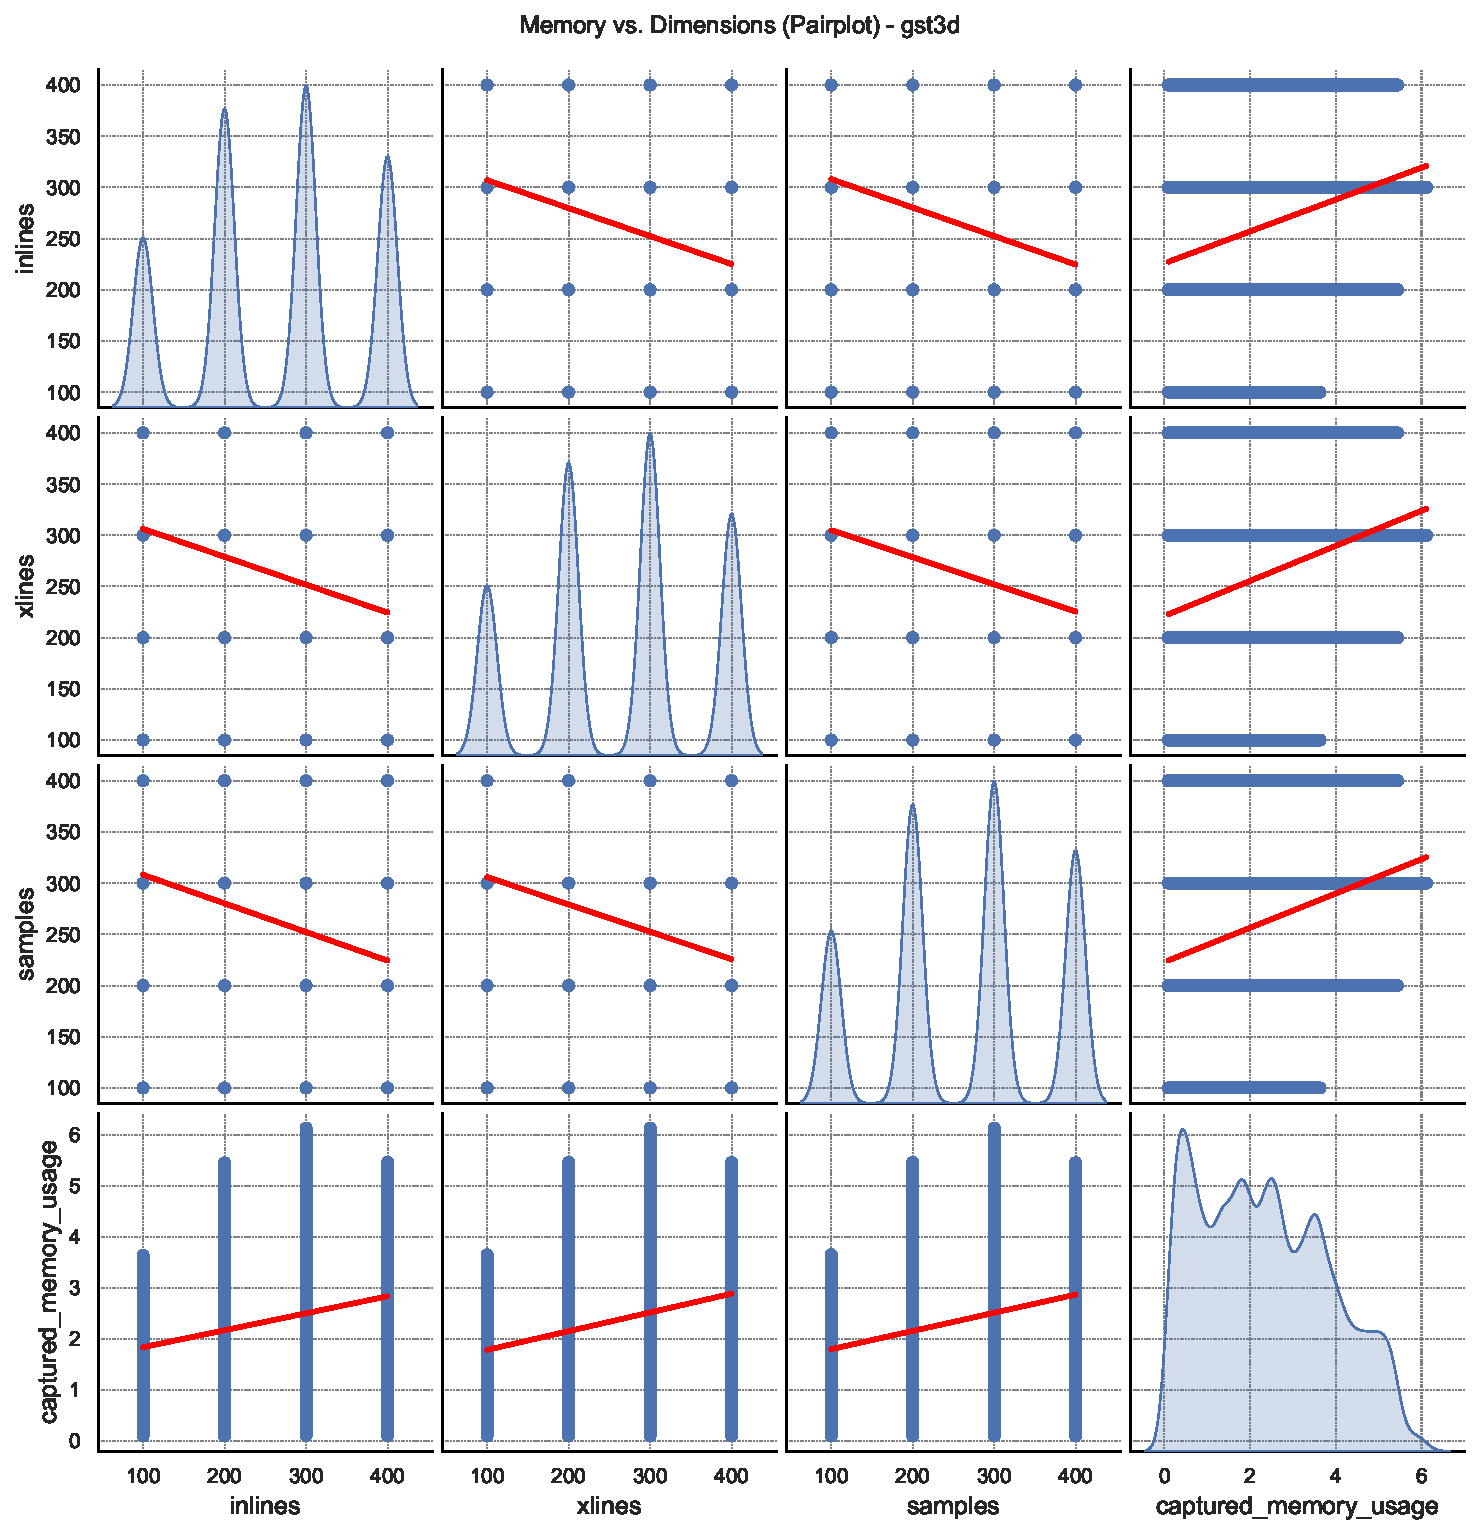
\includegraphics[width=0.9\textwidth]{assets/images/05/memory_vs_dimensions_pairplot_gst3d}
    \caption{Pairwise correlations for \ac{GST3D}. Memory usage rises with any dimension.}
    \label{fig:memory_vs_dimensions_pairplot_gst3d}
\end{figure}

\subsubsection{Summary of Observed Resource Usage}
\label{subsec:resource-usage-summary}

Table~\ref{tab:operator_summary_aggregates} summarizes volume ranges, memory usage, and execution time per operator.
\ac{GST3D} shows the highest resource usage, both in memory and time.
All operators reflect the volume-based trend discussed previously.

\begin{table}[htbp]
    \centering
    \begin{tabular}{lcccc}
        \hline
        \textbf{Operator} & \textbf{Volume Range}    & \textbf{Peak Mem. (GB)} & \textbf{Exec. Time (s)} \\
        \hline
        Envelope          & $10^6 \to 6.4\times10^7$ & 0.10 -- 1.76            & 0.0106 -- 0.5025        \\
        \ac{GST3D}        & $10^6 \to 2.7\times10^7$ & 0.31 -- 6.12            & 0.2475 -- 7.75          \\
        Gaussian Filter   & $10^6 \to 6.4\times10^7$ & 0.10 -- 0.57            & 0.0232 -- 1.22          \\
        \hline
    \end{tabular}
    \caption{Resource usage summary for Envelope, \ac{GST3D}, and Gaussian Filter. Volume is in number of elements.}
    \label{tab:operator_summary_aggregates}
\end{table}
